%% ERCAudit -- ICSE tool paper. Format: IEEE conference, 10pt (IEEEtran), PDF, at most 4 pages INCLUDING references.
%% Compile: pdflatex main.tex (twice) or tectonic -X compile main.tex. The bibliography is embedded.
%% The paper presents ONE tool (ERCAudit).
%% TODO before submission: \videourl, author list/affiliations, anonymisation if the track is double-blind, artifact DOI.
\documentclass[10pt,conference]{IEEEtran}

\usepackage{amsmath,amssymb}
\usepackage{graphicx}
\usepackage{booktabs}
\usepackage{multirow}
\usepackage{listings}
\usepackage{xcolor}
\usepackage{url}
\def\UrlBreaks{\do\/\do\_\do\-\do\.}
\Urlmuskip=0mu plus 1mu\relax
\usepackage[hidelinks]{hyperref}
\usepackage{cleveref} % should load this after hyperref/amssymb/etc.
\usepackage{balance}
\usepackage{tikz}
\usepackage{array}
\usepackage{wasysym}
\usepackage{makecell}
\usepackage{wasysym}
\usepackage{colortbl}
\usepackage{comment}
\usepackage{placeins}
\usepackage{xspace}
\usepackage[shortlabels]{enumitem}
\usetikzlibrary{arrows.meta,positioning,calc,fit}

% for comments
\usepackage{todonotes} % \usepackage[disable]{todonotes}
\newcommand{\fixme}[1]{\todo[inline,color=red!20,size=\footnotesize]{#1}}
\newcommand{\rev}[1]{{\color{blue}{#1}}} % \newcommand{\rev}[1]{#1}
\newcommand{\as}[1]{\textcolor{blue}{#1}}
\newcommand{\AS}[1]{\textcolor{orange}{#1}}

\newcommand{\tool}{\textsc{ERCAudit}\xspace}
\newcommand{\code}[1]{\texttt{#1}\xspace}
\newcommand{\us}{\_\allowbreak}
\newcommand{\gh}[1]{\footnote{\scriptsize\url{https://github.com/BatchTransfer/ERCAudit/blob/main/#1}}}
\newcommand{\ghtwo}[2]{\footnote{\scriptsize\url{https://github.com/BatchTransfer/ERCAudit/blob/main/#1}, \url{https://github.com/BatchTransfer/ERCAudit/blob/main/#2}}}
\newcommand{\artifacturl}{\url{https://github.com/BatchTransfer/ERCAudit}\xspace}   % TODO: final URL / Zenodo DOI
\newcommand{\videourl}{\url{https://www.youtube.com/watch?v=bvV_QXwJlp4}\xspace} 
\newcommand{\livedemo}{\url{https://batchtransfer.github.io/ERCAudit/}\xspace} % TODO: <= 5 min screencast

\lstdefinestyle{sh}{basicstyle=\ttfamily\fontsize{6.2}{7.0}\selectfont, breaklines=true, columns=fullflexible,
  keepspaces=true, xleftmargin=0pt, showstringspaces=false, aboveskip=2pt, belowskip=0pt, frame=tb, framerule=0.2pt,
  rulecolor=\color{black!50}}

\setlength{\textfloatsep}{6pt plus 2pt minus 2pt}\setlength{\floatsep}{5pt plus 2pt minus 2pt}\setlength{\intextsep}{5pt plus 2pt minus 2pt}\setlength{\abovecaptionskip}{2pt}\setlength{\skip\footins}{5pt plus 2pt minus 2pt}


\begin{document}

\title{\tool: Specification-Guided Auditing of ERC\\Implementations, from Standards to Deployments}

\author{\IEEEauthorblockN{Ashok Kasthuri and Lingxiao Jiang}
\IEEEauthorblockA{Singapore Management University, Singapore} 
% \\ashokk.2022@phdcs.smu.edu.sg}
}

\maketitle

\pagestyle{plain}
\thispagestyle{plain}

\begin{abstract}
\rev{Ethereum token standards (ERCs) describe how token contracts should behave, but many security requirements are written in prose and are not enforced by a compiler. 
We study two important cases: batch transfers, which move multiple tokens in one operation, and token approvals authorized by digital signatures. A missing transfer check can affect many tokens at once; a signature that is not bound to the intended contract and blockchain may be accepted in the wrong context.

We present \tool, an open-source tool that reformulates requirements for ERC-1155 batch transfers and EIP-712/ERC-2612 signature-based approvals into 17 executable checks, grouped into ten risk classes. Its compiler-independent source analyzer follows relevant contract logic across helper functions, initialization code, and cached state. 
Warnings generated by \tool checks are then validated against deployed contracts using transaction replay and signature-domain tests on testnets.
%, including tests that change the chain identifier.

\fixme{may shorten some of the technical details above and the experimental results below if space is tight.}
Across four EVM-compatible blockchains,
% (Ethereum, BNB Chain, Polygon, and Avalanche), 
\tool analyzed 35,406 batch-transfer implementations and flagged 915 potential errors. Among 148,517 verified-source contracts with permit-related functionality, it found 17,645 contracts violating at least one rule, producing 19,298 rule-level findings. On-chain tests confirmed 26 deployed tokens whose \texttt{permit} function did not verify a signature; 7,438 of 7,651 decidable stale-separator cases (97\%) kept a cached signature separator after the chain identifier changed. These results show how translating standards into checks and testing findings against deployed contracts can reveal security gaps that general-purpose analysis may miss. \tool's code \& datasets are available at \artifacturl; Video: \videourl; Live demo: \livedemo.
}
\end{abstract}

\begin{comment}
ERC standards describe token and signing behaviour in prose, so their security-critical requirements stay implicit: who may move
tokens, what a recipient must acknowledge, and which chain and contract a signature binds. A single missing validation in a batch
transfer can misdirect or destroy many tokens at once. A signing domain that omits or mis-builds its binding lets the same valid
signature be accepted by an unintended contract or chain, even though the signer is recovered correctly. 






We present \tool{}, an open-source tool that turns these requirements into source-level checks and validates the findings on chain. ERCAudit is a specification-guided auditor. It turns the requirements of ERC standards into executable source-level rules, 17 rules in ten risk classes for ERC-1155 batch transfers and EIP-712 / ERC-2612 signing domains, and then confirms or refutes each finding on the deployed contract. The analyzer works without a compiler. It follows how a contract builds its transfer logic and signing domain across helpers, initializers and cached state.


% \todo{is it really "one command and one report", in what sense? what's its significance?} behind one command and one report. 
% \tool{} reports\fixme{the word "reports" isn't clear what's novel; better to have a sentence or two to explain the novelty and significance of your tool, and then say it reports...}
% \textbf{ten risk classes}: five for ERC-1155 batch transfers (eight constraints) and five
% authority boundaries for EIP-712/ERC-2612 signing domains (nine rules, R1--R9). 

On-chain analysis---transaction replay, separator recomputation and a chain-ID fork test---confirms or refutes each finding. In our study of four EVM chains, \tool{} identified 35{,}406 batch-transfer
implementations, 915
% \fixme{is this number counted at contract level or rule-level?} 
of which are reported to contain errors, and analysed 148{,}517 permit-related contracts, reporting 19{,}298
% \fixme{are these numbers rule-level or also contract-level like 148,517? Need to be clear; this is unclear until very later when \Cref{tab:taxonomy-by-chain} is shown} 
risks both are at rule level.
On-chain evidence confirms, for example, 26 deployed tokens whose \code{permit} checks no signature and 97\% of the decidable stale-separator
cases. Code, data and video: \artifacturl{}\\
\videourl\\
\livedemo.
\end{comment}

\begin{IEEEkeywords}
smart contracts, ERC standards, static analysis, specification-guided auditing, on-chain validation
\end{IEEEkeywords}

%% =====================================================================
\section{Introduction}
ERC standards define how tokens and signatures should behave on Ethereum, but a standard is only a written description and a code interface, so nothing forces an implementation to follow it.
The compiler only checks the interface and leaves the properties that protect users to the implementer. 
For example, an ERC-1155 batch transfer must
authenticate the caller, reject the zero address, compare array lengths and confirm that a contract recipient accepted the
tokens~\cite{erc1155:misc}. An EIP-712 verifier must bind a signature to the active chain and to itself~\cite{eip712,eip2612}.
Violations of such constraints can be silent because the contract implementation can still compile and be used to move tokens. One omitted check can affect many assets in one call, and a wrongly bound
signing domain could let one valid signature authorize an action on another contract or chain.

General-purpose analyzers~\cite{feist2019slither,tsankov2018securify,luu2016making} look for generic defects and do not encode these ERC-specific
constraints. We present \tool{} to address this gap. \textbf{Contributions.}
% AS: novelty fixme addressed in the items below (marked in orange).
\begin{itemize}[leftmargin=*]
\item \textbf{Problem and rules.} We turn the specifications into \AS{rules} for ERC implementations: eight for batch transfers and, for signatures, nine source-level rules in five authority boundaries, which together give ten risk classes. \AS{We derive them by hand, so each rule traces to the normative text or, for R2--R9, to security considerations\gh{docs/RULES.md}; no tool in \cref{tab:related-work-comparison} covers domain freshness or the logical domain.}
\item \textbf{\tool{}.} We build one specification-guided static analyzer with a shared front-end that follows transfer logic and domain construction across helpers, initializers, and cached state, and reports each finding with its rule, class, severity, and evidence in one schema. \AS{It needs no compiler (median 8\,ms per batch and 50\,ms per permit contract).}
\item \textbf{Large-scale study and dataset.} In our study we analyze 35{,}406 batch-transfer implementations (915 risks) and 148{,}517 permit-related contracts (19{,}298 risks) on Ethereum, BNB Chain, Polygon and Avalanche, report verified findings, and demonstrate controlled testnet exploits and a replay.
\item \textbf{On-chain verification.} We check flagged contracts against deployed state and real executions by replaying batch-transfer transactions, rebuilding separators, decoding deployment arguments, simulating permits, and forking chains under a changed identifier.\AS{On chain, 7{,}949 domain findings are confirmed and 1{,}257 refuted (979 are R4 candidates with a correct chain ID); the rest stay unresolved (\cref{tab:dom}).}

\end{itemize}



% AS: Figure fig:replay moved into Section Design, next to the signing-domain rules it illustrates.

\begin{figure*}[t]
\centering
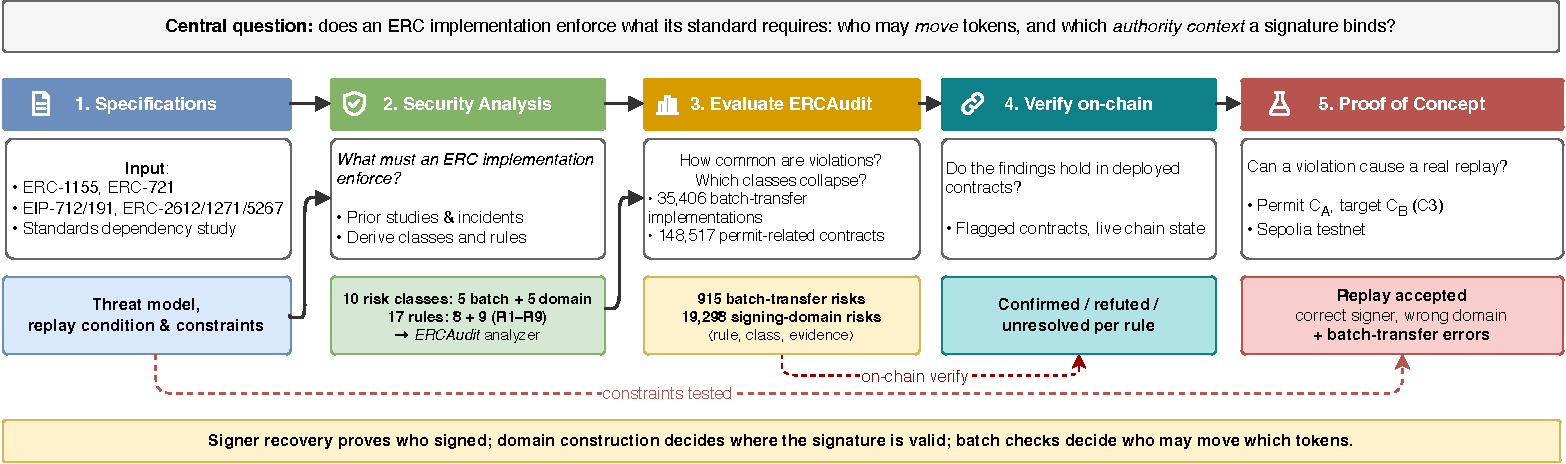
\includegraphics[width=0.9\textwidth]{fig_overview.pdf}
\caption{Overview of \tool{}: from the specifications to ten risk classes and 17 rules, their evaluation on two corpora, on-chain verification and proof-of-concept experiments.}

\label{fig:overview}
\end{figure*}




% AS: former section 'Threat Model for Signing Domains' merged into Section Design (signing-domain rules), as the comments suggested.

%% =====================================================================
\section{Design}
\label{sec:design}
\textbf{Overview (Fig.~\ref{fig:overview}).} \tool{} \footnote{\scriptsize Artifact: \url{https://github.com/BatchTransfer/ERCAudit} \\ \hspace*{1em} Video: \url{https://www.youtube.com/watch?v=bvV_QXwJlp4} \\ \hspace*{1em} Live demo, runs in the browser: \url{https://batchtransfer.github.io/ERCAudit/}} works in five steps. (1)~\emph{Specifications}: we derive \AS{rules} from the text of
ERC-1155 and ERC-721, EIP-712/191 and ERC-2612/1271/5267, and from a study of how these standards depend on each other. % AS: json footnote moved to stage P1
We evaluate rule sets for ERC-1155 and EIP-712/ERC-2612.
(2)~\emph{Security analysis}: we group the requirements into ten risk classes and 17 rules (eight batch-transfer \AS{rules} and nine signing-domain
rules). % AS: code footnotes moved to the rule-set paragraph
(3)~\emph{Evaluation}: we run the rules on \AS{a batch-transfer corpus and a permit-related corpus (\cref{sec:eval}).} % AS: results removed from the overview
(4)~\emph{On-chain verification}: we check flagged contracts against deployed state and real transactions. (5)~\emph{Proof of concept}:
our testnet experiments show a replay accepted under a correct signer and a wrong domain, and batch-transfer errors that burn or misroute tokens.

\begin{table}[t]
\caption{Batch-transfer rule set: the eight rules of ERC-1155 \code{safeBatchTransferFrom} and the risk class each populates.}
\label{tab:batch}
\centering\scriptsize\setlength{\tabcolsep}{2pt}
\begin{tabular}{@{}l l >{\raggedright\arraybackslash}p{3.2cm}@{}}
\toprule
Risk class & Rule & Formal definition\\\midrule
B1 access control & Authorization & $\textit{sender}=\textit{from}\ \lor$ \textit{isApprovedForAll(from, sender)}\\
B2 address validation & Recipient validity & $\textit{to}\neq 0\text{x}0$\\
-- & Balance sufficiency & $\forall i:\textit{balanceOf(from,id}_i)\!\geq\!\textit{val}_i$\\
B3 array-length check & Array integrity & $|\overrightarrow{\textit{ids}}|=|\overrightarrow{\textit{values}}|>0$\\
-- & Atomicity & $\mathcal{S}'=\mathcal{S}$ if any internal transfer fails\\
B4 event inconsistency & Event emission & emit \textit{TransferBatch}(\ldots) after the transfer\\
B5 interface check & Interface compliance & $\mathrm{IsContract}(\textit{to})\Rightarrow$ receiver returns magic value\\
-- & Gas efficiency & $\mathcal{G}(\overrightarrow{\textit{ids}})\leq \mathcal{G}_{\text{block}}$ $\wedge$ $\mathcal{G}(\overrightarrow{\textit{ids}})\leq\sum_i\mathcal{G}(\textit{id}_i)$\\
\bottomrule
\end{tabular}
% AS: normative basis, preconditions, false positives and on-chain decidability are in docs/RULES.md (linked below).
\end{table}


\begin{table}[t]
\caption{Signing-domain rules R1--R9 in five authority boundaries (classes).}
\label{tab:domain-risk-rules}
\centering\scriptsize\setlength{\tabcolsep}{2pt}
\newcolumntype{L}[1]{>{\raggedright\arraybackslash}p{#1}}
\begin{tabular}{@{}L{3.3cm} L{4.8cm}@{}}
\toprule
Rule & Requirement\\\midrule
\rowcolor{black!12}\multicolumn{2}{l}{\textbf{C1 Domain separation}}\\
\hspace{1.4em}R1 Missing separator & Digest has separator and \code{0x1901} prefix\\
\rowcolor{black!12}\multicolumn{2}{l}{\textbf{C2 Chain binding}}\\
\hspace{1.4em}R2 Missing \code{chainId} & Domain includes the chain ID\\
\hspace{1.4em}R3 Hard-coded \code{chainId} & Chain ID is not a fixed constant\\
\hspace{1.4em}R4 Deployed \code{chainId} & Passed ID equals the deployed chain\\
\rowcolor{black!12}\multicolumn{2}{l}{\textbf{C3 Verifier binding}}\\
\hspace{1.4em}R5 Missing verifier & Domain includes the verifier address\\
\hspace{1.4em}R6 Hard-coded verifier & Verifier is \code{address(this)}, not a literal\\
\hspace{1.4em}R7 External verifier & Passed verifier is the contract itself\\
\rowcolor{black!12}\multicolumn{2}{l}{\textbf{C4 Domain freshness}}\\
\hspace{1.4em}R8 Stored separator & Recomputed when context changes\\
\rowcolor{black!12}\multicolumn{2}{l}{\textbf{C5 Logical domain}}\\
\hspace{1.4em}R9 Hard-coded salt & Salt is not zero or shared\\
\bottomrule
\end{tabular}
\end{table}

\textbf{From specification to \AS{rules}.} \AS{A \emph{rule} is one requirement taken from a standard, a \emph{rule set} is the rules of one standard (batch transfer or signing domain), and a \emph{constraint} is the boolean check of a rule over extracted facts.} A rule set defines the \emph{facts} we extract, the boolean \emph{constraints} over
them, the mapping to \emph{risk classes} with severity, and the \emph{evidence} we report. 

We encode a set of eight \AS{rules} for batch-transfer in Table~\ref{tab:batch}, which follow the canonical batch-transfer workflow.\AS{\ghtwo{ercaudit/batchaudit/constraints.py}{ercaudit/domaudit/rules.py}}


Five of them (1, 2, 4, 6, 7) are checked statically through eight source-level predicates and
populate the five classes B1--B5. 
\AS{\gh{docs/RULES.md} gives each rule's normative basis, preconditions, expected false positives and on-chain decidability. Batch rules 1, 2, 4, 6 and 7 come from MUST statements of ERC-1155.}

We also encode a set of nine rules for signing domain on how a contract builds, stores and exposes its
EIP-712 domain (Table~\ref{tab:domain-risk-rules}), grouped into five authority boundaries C1--C5. 
\AS{Only R1 follows from the EIP-712 digest encoding; R2--R9 are recommended practice, since EIP-712 makes every domain field optional.}

\AS{\textbf{Signing domains and threat model.} A \emph{signing domain} is the data (name, version, chain ID, verifier, salt) that EIP-712 hashes into each typed-data signature; it exists only for EIP-712-based standards such as ERC-2612, ERC-1271 and ERC-5267. The model below is background that justifies R1--R9 only; the batch rules follow from the ERC-1155 text and need no adversary.}

\textbf{Adversary.} The attacker obtains a valid typed-data signature $\sigma=(v,r,s)$ and its signed message $m$, for example from public calldata or a relay workflow, or from any other channel the signed payload travels through. The attacker can deploy contracts and submit arbitrary transactions. The attacker cannot forge signatures, steal keys, alter deployed code, or skip the target's own checks, which include signer recovery, nonce, and deadline~\cite{meisami2025sigscope}. A violation is therefore a \emph{replay condition} and not an exploit, because exploitation also needs a state-changing target that accepts the replayed authorization.

\textbf{Replay condition.} 
% AS: threat-model fixme addressed by merging this text into Design.
Let the signer intend authority context $\mathcal{A}_S$ for a source verifier $V_S$, and let a target verifier $V_T$ operate in context $\mathcal{A}_T$. A context bundles the four boundaries a signature should respect: $\mathcal{A}=\langle \mathit{chain},\mathit{verifier},\mathit{freshness},\mathit{logicalDomain}\rangle$, where \emph{freshness} covers deployment, proxy, upgrade, and cache state. Replay at $V_T$ succeeds iff
\begin{equation}
\label{eq:failure}
\mathcal{A}_S\neq\mathcal{A}_T\;\land\;\delta_{\mathcal{A}_S}(m)=\delta_{\mathcal{A}_T}(m)\;\land\;\textsc{LocalChecks}_{V_T}(m,\sigma),
\end{equation}
where $\delta_{\mathcal{A}}(m)=H(\texttt{0x1901}\parallel D(\mathcal{A})\parallel\texttt{hashStruct}(m))$ and \textsc{LocalChecks} covers nonce, deadline, and signer recovery. Nonces are local to each verifier, so consuming a nonce at $V_S$ does not consume it at $V_T$ (Figure~\ref{fig:replay}). Equivalently, let $W(\sigma)$ be the contexts the signer intends and $C(\sigma)$ the contexts in which deployed verifiers accept $\sigma$. Security requires $C(\sigma)\subseteq W(\sigma)$, and a \emph{signature-construction failure} is any verifier that accepts $\sigma$ outside $W(\sigma)$. Signer recovery proves \emph{who} signed and domain construction decides \emph{where} the signature is valid.

\begin{figure}[t]
\centering
\resizebox{\columnwidth}{!}{%
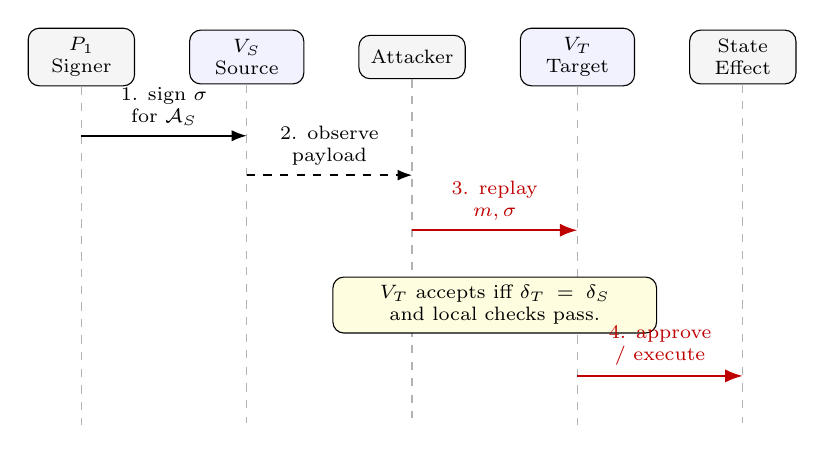
\begin{tikzpicture}[
    font=\scriptsize,
    >=Latex,
    lifeline/.style={dashed, gray!60, line width=0.45pt},
    actor/.style={draw, rounded corners, fill=gray!8, minimum width=1.35cm, minimum height=0.55cm, align=center},
    verifier/.style={draw, rounded corners, fill=blue!5, minimum width=1.45cm, minimum height=0.55cm, align=center},
    msg/.style={->, line width=0.55pt},
    obs/.style={->, dashed, line width=0.5pt},
    bad/.style={->, red!75!black, line width=0.75pt},
    note/.style={draw, rounded corners, fill=yellow!12, text width=3.9cm, align=center, inner sep=3pt}
]
\node[actor]    (p1) at (0,0) {$P_1$\\Signer};
\node[verifier] (vs) at (2.1,0) {$V_S$\\Source};
\node[actor]    (a)  at (4.2,0) {Attacker};
\node[verifier] (vt) at (6.3,0) {$V_T$\\Target};
\node[actor]    (st) at (8.4,0) {State\\Effect};
\foreach \n in {p1,vs,a,vt,st} { \draw[lifeline] (\n.south) -- ++(0,-4.3); }
\draw[msg] (p1.south |- 0,-1.0) -- node[above,align=center] {1. sign $\sigma$\\for $\mathcal{A}_S$} (vs.south |- 0,-1.0);
\draw[obs] (vs.south |- 0,-1.5) -- node[above,align=center] {2. observe\\payload} (a.south |- 0,-1.5);
\draw[bad] (a.south |- 0,-2.2) -- node[above,align=center,text=red!75!black] {3. replay\\$m,\sigma$} (vt.south |- 0,-2.2);
\node[note] at (5.25,-3.15) {$V_T$ accepts iff $\delta_T=\delta_S$\\and local checks pass.};
\draw[bad] (vt.south |- 0,-4.05) -- node[above,align=center,text=red!75!black] {4. approve\\/ execute} (st.south |- 0,-4.05);
\end{tikzpicture}%
}
\caption{Authority-boundary replay. The target recovers the correct signer in the wrong authority context.}
\label{fig:replay}
\end{figure}


\AS{Together the two rule sets give \textbf{ten risk classes}: five for batch transfers (B1--B5) and five for signing domains (C1--C5); gas is triaged manually and not counted.} Two
domain rules (R4, R7) are \emph{conditional}, because their safety depends on a value passed at deployment, so we report them as candidates for chain checks.

\textbf{\AS{Analyzer internals.}} \AS{Step (2) runs five internal stages, P1--P5.} P1 is a corpus-scale pre-filter that finds candidate contracts by selector: \code{0x2eb2c2d6} for batch transfers,
\code{0xd505accf} for \code{permit}, and \code{0x3644e515}, \code{0x84b0196e}, \code{0x1626ba7e} for domain, metadata and ERC-1271. \AS{The selectors of 79 ERCs come from a specification file\gh{data/specifications/final_basic_erc_specifications.json}.} P2 recovers functions by
brace matching and follows a bounded call graph. P3 extracts the
predicates that guard state changes (\code{require}, \code{if}$\ldots$\code{revert}) and facts such as aliases of \code{ids.length}, the
\code{chainId} and verifier placed in the domain, and whether the separator is cached or recomputed. P4 evaluates the rule set on the entry point and
its callees, so a check delegated to a helper still counts, and P5 maps violations to classes, severities and evidence. P2--P4 need no compiler, so they also run on
flattened or multi-file Etherscan sources that the local toolchain cannot build.

\textbf{On-chain analysis.} Static findings say that a check is absent but not whether the deployed contract is affected, so we validate them on chain. For batch transfers we
fetch the \code{txlist} of flagged ERC-1155 contracts, decode the calldata offline and test three patterns: zero-address recipients,
length mismatch, and callers without a recorded approval. We also follow \code{setApprovalForAll} chains. For signing domains,
the deployed contract holds the answer. Our probes read or rebuild \code{DOMAIN\us SEPARATOR} with candidate field layouts (a keccak
match proves which fields the live domain binds), fork the chain twice with a different chain ID (R8), decode deployment arguments (R4),
and simulate \code{permit} with a throwaway key through a read-only \code{eth\us call} (R1).\gh{ercaudit/txaudit/patterns.py}

\rev{\textbf{Tool Usage.}
A developer runs \code{ercaudit audit TokenSample.sol}. Each finding gives the rule set, severity, rule and source lines, for example “domain High R3 hardcoded chainId”, and the exit status is 1 if anything is found, so the command can gate CI.

\AS{For a directory, \code{ercaudit audit DIR} applies every rule set, and \code{ercaudit run --size 100} runs the bundled sample and writes findings.csv with the stored on-chain verdicts.} 

The live demo (\livedemo) does the same in the browser: choose an example or paste a contract, press `Audit' button, and read the findings. 
%A finding is a violated rule, not a proven exploit.
}

% \fixme{because it's a tool demo paper, we should have a subsection with a few paragraphs to describe how to use/run the tool, giving some concrete commands like your video showed or briefly mention how to use the live demo and how to read/understand the report for a contract.}

% \fixme{since you have the live demo, it'd be better for the video to demonstrate show how a user can uses the live demo too. If time allows, please add this into the video.}

%% =====================================================================

%% =====================================================================
\section{Empirical Evaluation}
\label{sec:eval}
% \emph{Artifact.} \artifacturl{} (video: \videourl{}).\footnote{\scriptsize Live demo, runs in the browser: \url{https://batchtransfer.github.io/ERCAudit/}}
Our empirical study  evaluates: what does \tool{} find at scale, and does chain evidence confirm it?


\fixme{A note: this paper is for tool demo, so it's not necessary to write it as a “large-scale research study”; some of the results/tables may be omitted if can't be explained clearly. It'd be more important to show an easy-to-run tool, a compelling
end-to-end demonstration, a stable artifact/dataset, and credible operational evidence (even though not large-scale).}

\subsection{Findings and on-chain confirmation}
\AS{\textbf{Setup.} The batch corpus has 35{,}406 ERC-1155 batch-transfer implementations on four chains (\cref{tab:wholedataset}), 9{,}275 (26.19\%) with verified source, i.e.\ published on Etherscan; the domain corpus has 322{,}933 signature-related contracts (\cref{tab:corpus}). \emph{Permit-related} means the contract exposes EIP-712, ERC-2612, ERC-5267 or ERC-1271 features and \emph{violating} means it breaks at least one rule. We labelled 941 batch and 180 flagged domain contracts by hand, took sources and deployment arguments from Etherscan V2 and chain data from public RPC and Foundry anvil forks, and ran the analysis on a 32-core AMD EPYC 7542 server.}
\fixme{AS: please confirm the machine, the label counts (941, 180) and the data sources in the Setup paragraph.}

\begin{table}[tb]
  \centering
  \caption{Batch Transfer Dataset Overview}
  \label{tab:wholedataset}
  \footnotesize
  \setlength{\tabcolsep}{3.5pt}
  \renewcommand{\arraystretch}{1.15}
  \begin{tabular}{|p{1.4cm}|c|c|c|c|}
    \hline
    \textbf{Blockchain} &
    \textbf{\begin{tabular}[c]{@{}c@{}}Batch Transfer\\Count\end{tabular}} &
    \textbf{TVL} &
    \textbf{\begin{tabular}[c]{@{}c@{}}Total\\Transactions\end{tabular}} &
    \textbf{\begin{tabular}[c]{@{}c@{}}Available Code\\Count (\%)\end{tabular}} \\ \hline \hline

    Ethereum & 9,914 & \$3B & 9,772,654 & 5,608 (56.5\%) \\ \hline
    BNB Chain & 6,803 & \$821M & 1,116,248 & 1,666 (24.5\%) \\ \hline
    Avalanche & 1,023 & \$94M & 804,341 & 103 (10\%) \\ \hline
    Polygon & 17,666 & \$693M & 1,204,773 & 1,898 (10.7\%) \\ \hline
    \textbf{Total} & \textbf{35,406} & \textbf{\$4.6B} & \textbf{12,898,016} & \textbf{9,275 (26.19\%)} \\ \hline
  \end{tabular}
\end{table}

\begin{table}[tb]
  \centering
  \caption{Vulnerability Distribution by Type and Blockchain}
  \label{tab:report}
  \setlength{\tabcolsep}{2pt} % adjust horizontal spacing
  \renewcommand{\arraystretch}{1.0} % adjust row height
  {\scriptsize
  \begin{tabular}{|p{2.9cm}|c|c|c|c||c|}
    \hline
    \textbf{Vulnerabilities} &
    \textbf{Ethereum} &
    \textbf{BNB Chain} &
    \textbf{Avalanche} &
    \textbf{Polygon} &
    \textbf{Subtotal} \\ \hline \hline

    Missing Access Control & 35 & 9 & 0 & 3 & 47 \\ \hline
    Missing Address Validation & 143 & 21 & 1 & 48 & 213 \\ \hline
    Missing Array Length Check & 105 & 13 & 2 & 55 & 175 \\ \hline
    Event Emit Inconsistencies & 163 & 0 & 0 & 5 & 168 \\ \hline
    Missing Interface Check & 146 & 36 & 2 & 44 & 228 \\ \hline
    Gas-related Vulnerabilities & 59 & 11 & 0 & 14 & 84 \\ \hline \hline
    Total & 651 & 90 & 5 & 169 & 915 \\ \hline
  \end{tabular}
  }
\end{table}

\begin{table}[tb]
\centering
\scriptsize
\caption{Corpus and prevalence. Signature-related, typed-data (EIP-712), and permit (ERC-2612) columns count contracts with the feature, and \AS{violating} contracts violate at least one rule.}
\label{tab:corpus}
\setlength{\tabcolsep}{2.6pt}
\begin{tabular}{@{}p{1.2cm}p{1.2cm}p{1cm}p{1cm}p{1cm}p{1cm}r@{}}
\toprule
\textbf{Chain} & \textbf{Sig.-rel.} & \textbf{EIP-712} & \textbf{ERC-2612} & \textbf{\AS{Verified source}} & \textbf{\AS{Violating}} & \textbf{Rate} \\
\midrule
Ethereum  & 65,036  & 61,215  & 46,238 & 36,982  & 3,553  & 9.6\%  \\
BNB Chain & 105,025 & 102,341 & 84,029 & 52,114  & 7,481  & 14.4\% \\
Polygon   & 131,583 & 122,699 & 91,780 & 53,375  & 5,194  & 9.7\%  \\
Avalanche & 21,289  & 20,361  & 17,289 & 6,046   & 1,417  & 23.4\% \\
\midrule
\textbf{Total} & \textbf{322,933} & \textbf{306,616} & \textbf{239,336} & \textbf{148,517} & \textbf{17,645} & \textbf{11.9\%} \\
\bottomrule
\end{tabular}
\end{table}

\begin{table}[tb]
\centering
\scriptsize
\caption{Rule-level observations by chain. One contract may appear in several rules. Rule definitions are in Table~\ref{tab:domain-risk-rules}.}
\label{tab:taxonomy-by-chain}
\renewcommand{\arraystretch}{1.05}
\setlength{\tabcolsep}{1.6pt}
\begin{tabular}{p{2cm}p{1cm}p{1.1cm}p{1.1cm}p{1.1cm}p{1.1cm}}
\toprule
\textbf{Rule} & \textbf{Ethereum} & \textbf{BNB} & \textbf{Avalanche} & \textbf{Polygon} & \textbf{Total} \\
\midrule
\multicolumn{6}{l}{\emph{C1 Domain separation}} \\
R1 & 10 & 36 & 0 & 5 & 51 \\
\multicolumn{6}{l}{\emph{C2 Chain binding}} \\
R2 & 27 & 25 & 4 & 60 & 116 \\
R3 & 186 & 138 & 16 & 182 & 522 \\
R4 & 504 & 533 & 28 & 92 & 1{,}157 \\
\multicolumn{6}{l}{\emph{C3 Verifier binding}} \\
R5 & 31 & 5 & 0 & 22 & 58 \\
R6 & 76 & 37 & 6 & 51 & 170 \\
R7 & 87 & 83 & 14 & 78 & 262 \\
\multicolumn{6}{l}{\emph{C4 Domain freshness}} \\
R8 & 3{,}261 & 7{,}285 & 1{,}371 & 4{,}970 & 16{,}887 \\
\multicolumn{6}{l}{\emph{C5 Logical domain}} \\
R9 & 18 & 15 & 22 & 20 & 75 \\
\midrule
\textbf{Total} & \textbf{4{,}200} & \textbf{8{,}157} & \textbf{1{,}461} & \textbf{5{,}480} & \textbf{19{,}298} \\
\bottomrule
\end{tabular}
\end{table}

\begin{table}[tb]
\caption{Signing-domain rule set: rules R1--R9 in five authority boundaries (C1--C5), with static and on-chain results.
\AS{Confirmed = the violation holds on the deployed contract, Refuted = it does not, Unresolved = undecided; \Cref{tab:corpus} is static only.}}
\fixme{AS: terms now match \cref{tab:corpus}. Still open: R4 (1,157 vs 1,151) and R8 (16,887 vs 16,881) count source files while the on-chain columns count unique addresses, and the unresolved cells 149 and 9,236 are not in our data (143 and 9,230).}
\label{tab:dom}
\centering\scriptsize\setlength{\tabcolsep}{3pt}
\begin{tabular}{@{}l l r r r r@{}}
\toprule
Class & Rule & \AS{Violating} & \AS{Confirmed} & \AS{Refuted} & \AS{Unresolved}\\\midrule
C1 domain separation & R1 & 51 & 26 & 12 & 13\\
\multirow{3}{*}{C2 chain binding} & R2 & 116 & 76 & 0 & 40\\
 & R3 & 522 & 284 & 8 & 230\\
 & R4 & 1{,}157 & 29 & 979 & 149\\
\multirow{3}{*}{C3 verifier binding} & R5 & 58 & 15 & 0 & 43\\
 & R6 & 170 & 6 & 32 & 132\\
 & R7 & 262 & 72 & 13 & 177\\
C4 domain freshness & R8 & 16{,}887 & 7{,}438 & 213 & 9{,}236\\
C5 logical domain & R9 & 75 & 3 & 0 & 72\\\bottomrule
\end{tabular}
% \fixme{how is R4 1,151 different from 1,157 in \Cref{tab:taxonomy-by-chain}? R8 is also different: 16,881 vs. 16,887. Why?}
\end{table}


\textbf{Batch transfers.} In our study, \tool{} identified 35{,}406 batch-transfer implementations on four EVM chains (Table~\ref{tab:wholedataset}) and reports 915 of them with errors
(Table~\ref{tab:report}, with \AS{0.804 precision, i.e. 37 of the 46 flagged contracts in a hand-labelled sample of 941 were correct,} and 84 manually triaged gas issues). 

In ERC-1155, setApprovalForAll(operator, true) gives an operator control over all of the owner’s tokens. If that operator then approves further operators, authority spreads beyond what the owner granted, which breaks the authorization rule (B1). We follow such chains up to depth 5 among the transactions of flagged contracts and found 68 secondary-approval

% \fixme{not good to suddently mention "secondary-approval chains" without explanation; how are they related to the risks/vulnerabilities/ERC constraints?}

chains and no observed on-chain exploitation of length mismatches, and two testnet exploits (zero-address burn, length mismatch) show that violations can
destroy tokens.
\par\textbf{Signing domains.} 
% AS: experimental setting is now in the Setup paragraph above.
Across 148{,}517 \AS{verified-source} permit-related \AS{contracts} (Table~\ref{tab:corpus}), we found 17{,}645 contracts (11.9\%) that violate at least one rule, giving
19{,}298 rule-level observations (Table~\ref{tab:taxonomy-by-chain}), and freshness (R8) dominates by count. The final analyzer keeps 157 of 180 manually labelled flagged contracts
(89.8\% precision reported). On-chain evidence is our principal validation (Table~\ref{tab:dom}). It shows that 26 tokens (25 on BNB Chain) have a \code{permit} that verifies no signature, so
anyone can set any holder's allowance, that 76 of 116 R2 contracts bind no chain ID, that 29 of 1{,}151 R4 contracts (2.5\%) were deployed with a wrong chain ID
(16 with zero), and that 7{,}438 of 7{,}651 decidable R8 contracts (97\%) keep their cached separator when the chain ID changes. Pattern matching works for
syntactic rules (R2, R3, R5 and R9 reach 97--100\%) and fails when a rule encodes intent (R6 reaches 16\%), so we report such rules as review aids.

\FloatBarrier
%% =====================================================================
\section{Limitations and Related Work}
\textbf{Threats to validity.} \emph{Internal:} our tool is a static analysis method, so inheritance, wrappers and custom encodings cause
false positives and negatives. We have handled inline assembly to reduce false positives. We plan to add more such concrete patterns to reduce the false positives. we plan to complement our source-code analysis with bytecode-level analysis,
control-flow graph matching to better handle non-standard
implementations, wrapper functions, and proxy patterns \emph{Construct:} several rules approximate intent. Fixed chain identifiers, cached separators, and shared domains can be deliberate by design. Future work must dive deep into this intent way of construction and its purpose. \emph{External:} we analyze verified Solidity on four chains, so unverified bytecode, other languages,
standards and chains may differ, although the patterns are widely copied. 

\textbf{Related work.} Slither~\cite{feist2019slither}, Oyente~\cite{luu2016making} and Securify~\cite{tsankov2018securify} target generic defect classes, and \tool{} adds standard-specific constraints on similar primitives. Pied-Piper checks backdoors in ERC tokens~\cite{li2022pied},
and SymGPT audits contracts against ERC rules with symbolic execution and LLMs~\cite{xia2026symgpt}. SIGUARD, SigScope and OneSignature detect signature
defects and replay~\cite{zhang2023siguard,meisami2025sigscope,wang2025one}, whereas \tool{} checks how the domain itself is built and confirms findings on the deployed contract. Table~\ref{tab:related-work-comparison} compares \tool{} with these works\fixme{criteria for the comparison are unclear even though the table itself looks interesting; reviewers may view the table as superficial or unfair. better to make the criteria clearer; one sentence per comparator about the exact difference. Avoid over-claims or the impressions
about tools that have not been run or whose stated scope differs. If space is limited, can put the details (even the table itself) into a file in the repository and the paper just points to that link.} and with related studies of signature and cryptographic defects~\cite{wang2025copy,zhang2025demystifying,wang2026patterns}.

\begin{table}[tb]
\centering
\scriptsize
\caption{Comparison with related work. \CIRCLE: substantial coverage; \LEFTcircle: partial; \Circle: none. \AS{Marks follow each work's published scope; we did not re-run the tools.}}
\label{tab:related-work-comparison}
\setlength{\tabcolsep}{2pt}
\renewcommand{\arraystretch}{0.95}
\resizebox{\columnwidth}{!}{%
\begin{tabular}{@{}lccccccc@{}}
\toprule
\textbf{Work} & \makecell[c]{\textbf{Permit,}\\\textbf{ECDSA}} & \makecell[c]{\textbf{Domain}\\\textbf{sep.}} & \makecell[c]{\textbf{Chain}\\\textbf{binding}} & \makecell[c]{\textbf{Verifier}\\\textbf{binding}} & \makecell[c]{\textbf{Domain}\\\textbf{freshness}} & \makecell[c]{\textbf{Logical}\\\textbf{domain}} & \makecell[c]{\textbf{On-chain}\\\textbf{validation}} \\
\midrule
SigScope~\cite{meisami2025sigscope}      & \CIRCLE & \Circle & \Circle & \Circle & \Circle & \Circle & \Circle \\
Wang et al.~\cite{wang2025copy}          & \LEFTcircle & \Circle & \CIRCLE & \Circle & \Circle & \Circle & \Circle \\
OneSignature~\cite{wang2025one}          & \CIRCLE & \Circle & \CIRCLE & \CIRCLE & \Circle & \Circle & \Circle \\
Zhang et al.~\cite{zhang2025demystifying} & \LEFTcircle & \Circle & \LEFTcircle & \LEFTcircle & \Circle & \Circle & \Circle \\
SIGUARD~\cite{zhang2023siguard}          & \LEFTcircle & \LEFTcircle & \Circle & \Circle & \Circle & \Circle & \Circle \\
Wang et al.~\cite{wang2026patterns}      & \CIRCLE & \Circle & \CIRCLE & \CIRCLE & \Circle & \Circle & \Circle \\
{\bfseries\itshape ERCAudit}             & \LEFTcircle & \CIRCLE & \CIRCLE & \CIRCLE & \CIRCLE & \CIRCLE & \CIRCLE \\
\bottomrule
\end{tabular}%
}
\end{table}

\balance

\section{Conclusion}
We presented \tool{}, which makes ERC constraints executable and verifiable through one front-end, ten risk classes from replaceable rule sets, and an on-chain analysis that confirms or refutes each finding. In future work we plan a bytecode front-end for unverified contracts and re-labelled validation data for the final signing-domain rules.

% \appendices
\section*{Ethical Considerations}
\AS{\textbf{Computational cost.} The analysis takes a median of 8\,ms per batch and 50\,ms per permit contract on a laptop (Intel i7-9750H), and about 7\,s for the 200-contract sample; on-chain probes are dominated by network latency.}
Only public contract code, verified sources and public chain data are used. The on-chain probes use read-only calls and local forks, and our exploit demonstrations ran on testnets with our own contracts, so no live contract was exploited. Findings are constraint violations, not proven exploits.

\bibliographystyle{IEEEtran}
{\scriptsize\bibliography{refs}}

\end{document}
